\documentclass[11pt,a4paper]{article}
\usepackage[T1]{fontenc}
\usepackage[utf8]{inputenc}
\usepackage{lmodern}
\usepackage{textcomp}
\usepackage[left=1.8cm,right=1.8cm,top=3.0cm,bottom=2.2cm,headheight=36pt,headsep=12pt]{geometry}
\usepackage{multicol}
\usepackage{xcolor}
\usepackage{fancyhdr}\usepackage{tikz}
\usepackage{graphicx}
\usepackage{array}
\usepackage{amsmath,amssymb}
\usepackage{setspace}
\usepackage{longtable}
\graphicspath{{../}}
\definecolor{ygreen}{RGB}{46,139,87}\definecolor{dgreen}{RGB}{28,90,56}
\renewcommand{\normalsize}{\fontsize{10.9}{13.4}\selectfont}
\renewcommand{\familydefault}{\rmdefault}
\setlength{\parindent}{0pt}
\setlength{\columnsep}{0.8cm}
\setlength{\columnseprule}{0.4pt}
\setlength{\multicolsep}{3pt plus 1pt minus 1pt}
\renewcommand{\textsubscript}[1]{\ensuremath{_{\text{\fontsize{8}{8}\selectfont #1}}}}
\renewcommand{\textsuperscript}[1]{\ensuremath{^{\text{\fontsize{8}{8}\selectfont #1}}}}
\newcommand{\qn}[1]{\textbf{\fontsize{11.5}{13}\selectfont #1}}
\newcommand{\qsep}{\par\vspace{13pt}}
\newcommand{\fwrule}{\par\vspace{5pt}\noindent\rule{\linewidth}{1.4pt}\par\vspace{7pt}}
\newsavebox{\fitb}
\newcommand{\fitbox}[1]{\sbox{\fitb}{#1}\ifdim\wd\fitb>\linewidth\resizebox{\linewidth}{!}{\usebox{\fitb}}\else\usebox{\fitb}\fi}
\newcommand{\diqqat}[1]{\par\smallskip\noindent\textbf{Diqqat!} #1\par\medskip}
\newcommand{\javob}{\par\nopagebreak[4]\smallskip\noindent\textbf{Javob:} \rule[-2pt]{7.5cm}{0.4pt}\par\smallskip\noindent\textbf{Diqqat!} Javobingizni javoblar varaqasiga ko`chirib yozing.\par\medskip}
\pagestyle{fancy}
\fancyhf{}
\renewcommand{\headrulewidth}{1.6pt}\renewcommand{\headrule}{{\color{ygreen}\hrule height 1.6pt width\headwidth}}
\newcommand{\hdrlogo}{
\begin{tikzpicture}[baseline=0pt]\fill[ygreen,rounded corners=3pt] (0,0) rectangle (0.95,0.95);\node[white,font=\fontsize{24}{26}\bfseries\selectfont] at (0.475,0.47){K};\node[anchor=west,font=\fontsize{16}{18}\bfseries\selectfont,text=dgreen] at (1.15,0.66){KIMYO};\node[anchor=west,font=\footnotesize\scshape,text=gray] at (1.15,0.2){Milliy sertifikat\ \ 2026};\end{tikzpicture}}
\newcommand{\hdrpill}[1]{\begin{tikzpicture}[baseline=0pt]\node[fill=ygreen,text=white,rounded corners=8pt,inner xsep=10pt,inner ysep=5pt,font=\fontsize{13}{15}\bfseries\selectfont] at (0,0.475){#1};\end{tikzpicture}}
\fancyhead[L]{\hdrlogo}
\fancyhead[R]{\hdrpill{6-variant}}

\fancyfoot[C]{\thepage}
\fancypagestyle{first}{\fancyhf{}\renewcommand{\headrulewidth}{1.6pt}\renewcommand{\headrule}{{\color{ygreen}\hrule height 1.6pt width\headwidth}}\fancyhead[L]{\hdrlogo}\fancyhead[R]{\hdrpill{6-variant}}\fancyfoot[C]{\thepage}}
\begin{document}
\normalsize
\thispagestyle{first}
\noindent\textit{Davriy jadvaldan foydalanish mumkin.}
\par\smallskip
\begin{multicols}{2}
\noindent\qn{1.} Quyidagi moddalarning qaysilarida ion bog` mavjud? 1) (NH\textsubscript{4})\textsubscript{2}SO\textsubscript{4}; 2) NH\textsubscript{4}Cl; 3) H\textsubscript{2}O; 4) NaCl

\noindent A)~\textsl{1, 2, 4} \hfill B)~\textsl{1, 2, 3} \hfill C)~\textsl{3, 4} \hfill D)~\textsl{1, 3}\par
\qsep
\noindent\qn{2.} Rasmda kristall panjara tuzilishi tasvirlangan.
\begin{center}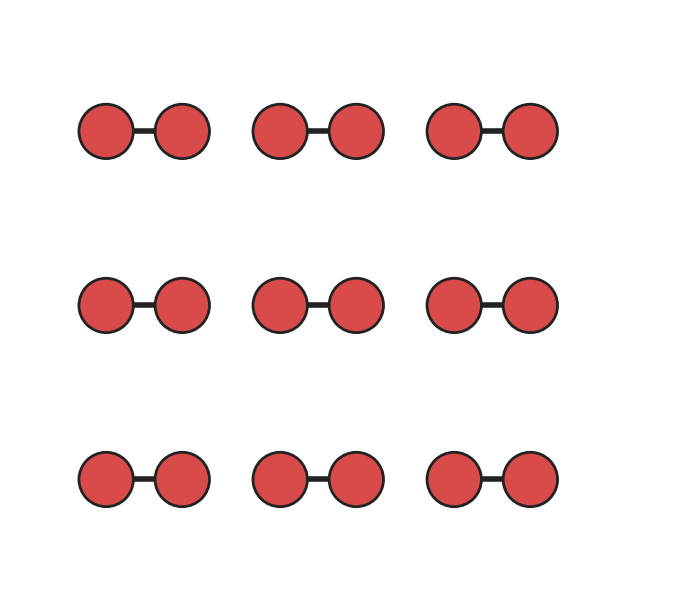
\includegraphics[width=0.86\linewidth]{rasmlar/gen/la_638325.png}\end{center}
Bu panjara qaysi turga kiradi?
\noindent A)~\textsl{ion kristall panjara}\par
\noindent B)~\textsl{molekulyar kristall panjara}\par
\noindent C)~\textsl{atom kristall panjara}\par
\noindent D)~\textsl{metall kristall panjara}\par
\qsep
\noindent\qn{3.} CuCl\textsubscript{2} ning suvli eritmasi inert elektrodlar bilan elektroliz qilinganda qaysi moddalar ajraladi?

\noindent\begin{tabular}{@{}p{0.47\linewidth}@{}p{0.47\linewidth}@{}}
A)~\textsl{Zn, H\textsubscript{2} va O\textsubscript{2}} & B)~\textsl{H\textsubscript{2}, Cl\textsubscript{2} va NaOH} \\
C)~\textsl{Cu va Cl\textsubscript{2}} & D)~\textsl{Ag va O\textsubscript{2}} \\
\end{tabular}\par
\qsep
\noindent\qn{4.} Kislorod (\textit{Z} = 8) atomida nechta juftlashmagan elektron bor?

\noindent A)~\textsl{2} \hfill B)~\textsl{3} \hfill C)~\textsl{1} \hfill D)~\textsl{4}\par
\qsep
\noindent\qn{5.} Quyidagi zarrachalardan qaysilari argon atomi bilan izoelektron? 1) Ca\textsuperscript{2+}; 2) N\textsuperscript{3$-$}; 3) Cl\textsuperscript{$-$}; 4) Mg\textsuperscript{2+}

\noindent A)~\textsl{3, 4} \hfill B)~\textsl{1, 4} \hfill C)~\textsl{1, 3} \hfill D)~\textsl{1, 2, 3}\par
\qsep
\noindent\qn{6.} Radioaktiv izotop yadrolari sonining vaqtga bog`liqligi grafikda berilgan.
\begin{center}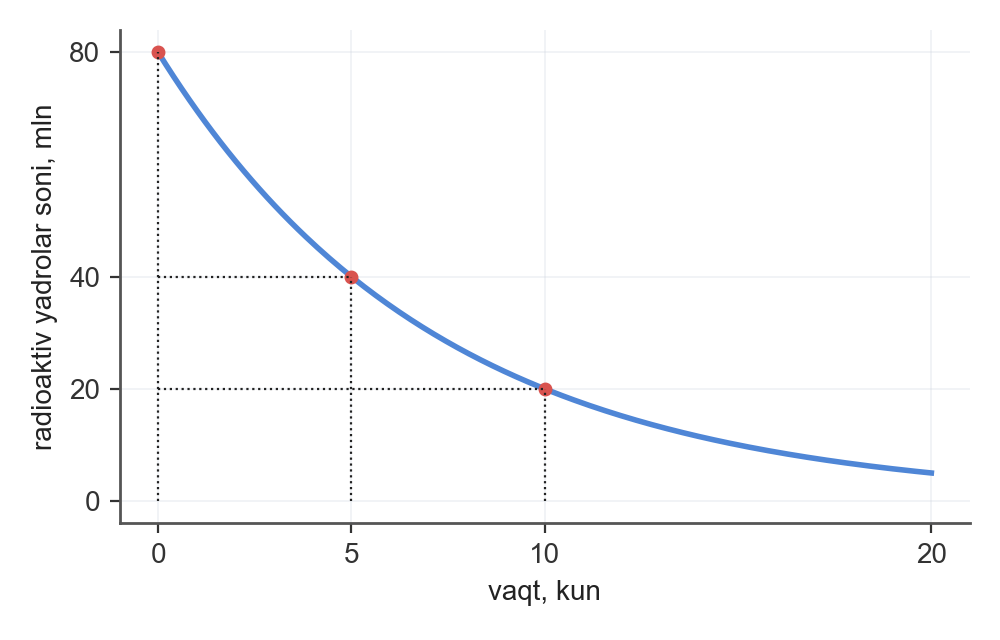
\includegraphics[width=0.86\linewidth]{rasmlar/gen/de_v06_0.png}\end{center}
4$\cdot$T vaqtdan keyin dastlabki yadrolarning necha foizi qoladi?

\noindent A)~\textsl{25} \hfill B)~\textsl{12,5} \hfill C)~\textsl{3,12} \hfill D)~\textsl{6,25}\par
\qsep
\noindent\qn{7.} Al + HNO\textsubscript{3} $\to$ Al(NO\textsubscript{3})\textsubscript{3} + NO + H\textsubscript{2}O reaksiya tenglamasini tenglang va barcha koeffitsiyentlar \textbf{yig`indisini aniqlang.}

\noindent A)~\textsl{10} \hfill B)~\textsl{8} \hfill C)~\textsl{11} \hfill D)~\textsl{9}\par
\qsep
\noindent\qn{8.} Fe plastinka CuSO\textsubscript{4} eritmasiga tushirildi. Reaksiya tugagach, plastinka massasi 0,8 g ga ortdi. Erigan Fe plastinka \textbf{massasini (g) aniqlang.}

\noindent A)~\textsl{6,4} \hfill B)~\textsl{0,8} \hfill C)~\textsl{11,2} \hfill D)~\textsl{5,6}\par
\qsep
\noindent\qn{9.} Metallning 5,6 g massasi oksidlanganda 7,2 g oksid hosil bo`ldi. Shu metallning 11,2 g miqdori kislotadan qancha hajm (l, n.sh.) vodorodni siqib chiqaradi? (Ekvivalent hajm \textit{V}\_E(H\textsubscript{2}) = 11,2 l/mol)

\noindent A)~\textsl{2,24} \hfill B)~\textsl{8,96} \hfill C)~\textsl{4,48} \hfill D)~\textsl{6,72}\par
\qsep
\noindent\qn{10.} Reaksiya tezligining harorat koeffitsiyenti $\gamma$ = 4. 20 \textdegree{}C da reaksiya 32 minutda tugasa, 60 \textdegree{}C da necha sekundda tugaydi?

\noindent A)~\textsl{7,5} \hfill B)~\textsl{491520} \hfill C)~\textsl{30} \hfill D)~\textsl{0,125}\par
\qsep
\noindent\qn{11.} N\textsubscript{2}O\textsubscript{5} moddaning parchalanish reaksiyasida konsentratsiyaning vaqt bo`yicha o`zgarishi jadvalda berilgan:
\begin{center}
\renewcommand{\arraystretch}{1.15}
\fitbox{\begin{tabular}{|c|c|}\hline
\textbf{t, min} & \textbf{c, mol/l} \\ \hline
0 & 1,6 \\ \hline
2 & 1,36 \\ \hline
4 & 1,12 \\ \hline
6 & 0,88 \\ \hline
\end{tabular}}
\end{center}
0-minutdan 6-minutgacha o`rtacha tezlikni mol/(l$\cdot$min) \textbf{hisoblang.}

\noindent A)~\textsl{0,12} \hfill B)~\textsl{0,24} \hfill C)~\textsl{0,06} \hfill D)~\textsl{0,72}\par
\qsep
\noindent\qn{12.} Noma'lum \textit{X} tuzining eruvchanligi (g/100 g suv) haroratga bog`liq jadvalda keltirilgan:
\begin{center}
\renewcommand{\arraystretch}{1.15}
\fitbox{\begin{tabular}{|c|c|c|c|c|}\hline
\textbf{t, \textdegree{}C} & \textbf{0} & \textbf{20} & \textbf{40} & \textbf{60} \\ \hline
S, g/100 g suv & 22 & 30 & 40 & 55 \\ \hline
\end{tabular}}
\end{center}
60 \textdegree{}C da tayyorlangan to`yingan 465 g eritma 20 \textdegree{}C gacha sovitildi. Cho`kmaga tushgan tuz \textbf{massasini (g) aniqlang.}

\noindent A)~\textsl{165} \hfill B)~\textsl{75} \hfill C)~\textsl{90} \hfill D)~\textsl{150}\par
\qsep
\noindent\qn{13.} C\textsubscript{2}H\textsubscript{6} $\rightleftarrows$ C\textsubscript{2}H\textsubscript{4} + H\textsubscript{2} reaksiyasi doimiy harorat va bosimda olib borildi; boshlang`ich modda qisman o`zgargach gazlar hajmi 6/5 marta ortdi. Boshlang`ich modda necha foizi \textbf{o`zgarganini aniqlang.}

\noindent A)~\textsl{10} \hfill B)~\textsl{20} \hfill C)~\textsl{40} \hfill D)~\textsl{80}\par
\qsep
\noindent\qn{14.} Qaysi juftliklar o`zaro reaksiyaga kirishadi? 1) SiO\textsubscript{2} va H\textsubscript{2}O; 2) Ag va H\textsubscript{2}SO\textsubscript{4}(suyult.); 3) MgCl\textsubscript{2} va KNO\textsubscript{3}; 4) Fe va HCl

\noindent A)~\textsl{2, 3} \hfill B)~\textsl{1} \hfill C)~\textsl{4} \hfill D)~\textsl{3, 4}\par
\qsep
\noindent\qn{15.} 11,2 l (n.sh.) ammiakdan nitrat kislota olindi (jami unum 90\%). Barcha reaksiyalar 1 atm bosimda olib borildi. Kislota \textbf{massasini (g) aniqlang.}

\noindent A)~\textsl{31,5} \hfill B)~\textsl{56,7} \hfill C)~\textsl{14,18} \hfill D)~\textsl{28,35}\par
\qsep
\noindent\qn{16.} Probirkalardagi eritmalar: Na\textsubscript{2}SO\textsubscript{4}, Na\textsubscript{2}CO\textsubscript{3}, NaCl ni alohida probirkalarda ajratish uchun qaysi reagent(lar) yetarli? 1) BaCl\textsubscript{2} va fenolftalein; 2) HCl va BaCl\textsubscript{2}; 3) fenolftalein; 4) lakmus va fenolftalein

\noindent A)~\textsl{4} \hfill B)~\textsl{2, 3, 4} \hfill C)~\textsl{3, 4} \hfill D)~\textsl{1, 2}\par
\qsep
\noindent\qn{17.} Si va SiO\textsubscript{2} dan iborat 8,8 g aralashma mo`l NaOH eritmasi bilan qizdirilganda 4,48 l (n.sh.) vodorod ajraldi. Reagent (NaOH) eritmasining massa ulushi 50\% va zichligi 1,18 g/ml; u mo`l miqdorda olingan. Aralashmani to`liq eritish uchun sarflangan NaOH \textbf{massasini (g) hisoblang.}

\noindent A)~\textsl{8} \hfill B)~\textsl{16} \hfill C)~\textsl{32} \hfill D)~\textsl{24}\par
\qsep
\noindent\qn{18.} Ca va CaC\textsubscript{2} dan iborat aralashma suv bilan ta'sirlashganda 8,96 l (n.sh.) gaz aralashmasi ajraldi, uning vodorodga nisbatan zichligi 7. Dastlabki aralashmaning \textbf{massasini (g) hisoblang.}

\noindent A)~\textsl{41,6} \hfill B)~\textsl{10,4} \hfill C)~\textsl{20,8} \hfill D)~\textsl{31,2}\par
\qsep
\noindent\qn{19.} NO va O\textsubscript{2} dan iborat 120 ml aralashma (hajmlar bir xil sharoitda) o`zaro ta'sirlashgandan so`ng hajmi 90 ml bo`lib qoldi (NO to`liq reaksiyaga kirishdi, kislorod ortiqcha). Dastlabki aralashmadagi NO ning hajmiy \textbf{ulushini (\%) aniqlang.}

\noindent A)~\textsl{50} \hfill B)~\textsl{66,67} \hfill C)~\textsl{25} \hfill D)~\textsl{100}\par
\qsep
\noindent\qn{20.} Alken, alkadiyen va alkinlar haqida qaysi fikrlar to`g`ri? 1) Alkinlar uchun umumiy formula CnH\textsubscript{2}n+2; 2) Kauchuk izoprenning polimeri; 3) Etilen bromli suvni rangsizlantiradi; 4) Alkenlarda $\pi$-bog` yo`q

\noindent A)~\textsl{1, 3, 4} \hfill B)~\textsl{3, 4} \hfill C)~\textsl{1, 3} \hfill D)~\textsl{2, 3}\par
\qsep
\noindent\qn{21.} Karbon kislotalar haqida qaysi fikrlar to`g`ri? 1) Benzoy kislota Na\textsubscript{2}CO\textsubscript{3} bilan reaksiyaga kirishmaydi; 2) Chumoli kislota "kumush ko`zgu" reaksiyasini beradi; 3) Sirka angidrid ikki molekula sirka kislotadan suv chiqib hosil bo`ladi; 4) Sirka kislota karbonatlar bilan CO\textsubscript{2} ajratadi

\noindent A)~\textsl{1, 3} \hfill B)~\textsl{2, 3, 4} \hfill C)~\textsl{1, 2, 4} \hfill D)~\textsl{1, 3, 4}\par
\qsep
\noindent\qn{22.} Quyidagi birikmalardan qaysi biri spirt sinfiga kiradi?

\noindent A)~\textsl{C\textsubscript{6}H\textsubscript{5}NH\textsubscript{2}} \hfill B)~\textsl{C\textsubscript{2}H\textsubscript{5}OH} \hfill C)~\textsl{CH\textsubscript{3}NO\textsubscript{2}} \hfill D)~\textsl{CH\textsubscript{3}COCH\textsubscript{3}}\par
\qsep
\noindent\qn{23.} 78 g benzol nitrolandi (unum 80\%), hosil bo`lgan nitrobenzol Zinin reaksiyasi bo`yicha qaytarildi (unum 90\%). Barcha reaksiyalar 1,5 atm bosimda olib borildi. Olingan anilin \textbf{massasini (g) hisoblang.}

\noindent A)~\textsl{67} \hfill B)~\textsl{133,9} \hfill C)~\textsl{33,5} \hfill D)~\textsl{93}\par
\qsep
\noindent\qn{24.} Formaldegid va propanal aralashmasi (7,3 g) mo`l ammiakli kumush oksid eritmasi bilan qizdirilganda 43,2 g kumush ajraldi. Qizdirish 60 daqiqa davom etdi. Aralashmadagi propanalning \textbf{massasini (g) aniqlang.}

\noindent A)~\textsl{5,8} \hfill B)~\textsl{1,5} \hfill C)~\textsl{11,6} \hfill D)~\textsl{3,7}\par
\qsep
\noindent\qn{25.} 180 g glukoza spirtli bijg`ishga uchradi (unum 80\%). Ajralgan gaz mo`l ohakli suvdan o`tkazilganda necha gramm cho`kma hosil bo`ladi?

\noindent A)~\textsl{200} \hfill B)~\textsl{80} \hfill C)~\textsl{320} \hfill D)~\textsl{160}\par
\qsep
\noindent\qn{26.} C\textsubscript{2}H\textsubscript{4} va C\textsubscript{3}H\textsubscript{8} aralashmasi tarkibida C\textsubscript{2}H\textsubscript{4} va C\textsubscript{3}H\textsubscript{8} ning massalari nisbati 14 : 33. Shu aralashmani yondirish uchun 47,04 l (n.sh.) kislorod sarflandi. Aralashmadagi C\textsubscript{2}H\textsubscript{4} ning \textbf{massasini (g) toping.}

\noindent A)~\textsl{13,2} \hfill B)~\textsl{5,6} \hfill C)~\textsl{11,2} \hfill D)~\textsl{9,4}\par
\qsep
\noindent\qn{27.} 120 g CH\textsubscript{3}COOH dan quyidagi sxema bo`yicha 42,07 g glitsilglitsin olindi: CH\textsubscript{3}COOH $\to$ ClCH\textsubscript{2}COOH $\to$ H\textsubscript{2}N--CH\textsubscript{2}--COOH $\to$ dipeptid. Dastlabki 2 bosqichning unumi ketma-ket 75\%, 50\% ga teng. Oxirgi bosqichning \textbf{unumini (\%) aniqlang.}

\noindent A)~\textsl{42} \hfill B)~\textsl{15} \hfill C)~\textsl{68} \hfill D)~\textsl{85}\par
\qsep
\noindent\qn{28.} 46 g C\textsubscript{2}H\textsubscript{5}OH dan quyidagi sxema bo`yicha 39,68 g etilenglikol olindi: C\textsubscript{2}H\textsubscript{5}OH $\to$ C\textsubscript{2}H\textsubscript{4} $\to$ HOCH\textsubscript{2}--CH\textsubscript{2}OH. Dastlabki 1 bosqichning unumi ketma-ket 80\% ga teng. Barcha reaksiyalar 1 atm bosimda olib borildi. Oxirgi bosqichning \textbf{unumini (\%) aniqlang.}

\noindent A)~\textsl{40} \hfill B)~\textsl{20} \hfill C)~\textsl{80} \hfill D)~\textsl{64}\par
\qsep
\noindent\qn{29.} 61,5 g C\textsubscript{6}H\textsubscript{5}NO\textsubscript{2} dan quyidagi sxema bo`yicha 27,52 g fenilammoniy xlorid olindi: C\textsubscript{6}H\textsubscript{5}NO\textsubscript{2} $\to$ C\textsubscript{6}H\textsubscript{5}NH\textsubscript{2} $\to$ [C\textsubscript{6}H\textsubscript{5}NH\textsubscript{3}]Cl. Dastlabki 1 bosqichning unumi ketma-ket 50\% ga teng. Barcha reaksiyalar 1 atm bosimda olib borildi. Oxirgi bosqichning \textbf{unumini (\%) aniqlang.}

\noindent A)~\textsl{42} \hfill B)~\textsl{85} \hfill C)~\textsl{15} \hfill D)~\textsl{68}\par
\qsep
\noindent\qn{30.} Kimyoviy laboratoriyada ajratgich voronka nima uchun ishlatiladi?
\noindent A)~\textsl{aralashmaydigan suyuqliklarni ajratish}\par
\noindent B)~\textsl{gaz (H\textsubscript{2}, CO\textsubscript{2}, H\textsubscript{2}S) olish}\par
\noindent C)~\textsl{vakuum ostida filtrlash}\par
\noindent D)~\textsl{eritmalarni bug`latish}\par
\qsep
\noindent\qn{31.} Rasmdagi asbobda 23 g etanol konsentrlangan H\textsubscript{2}SO\textsubscript{4} bilan 170 \textdegree{}C da qizdirilib, 90\% unum bilan etilen olindi. Hosil bo`lgan etilen \textbf{hajmini (l, n.sh.) aniqlang.}
\begin{center}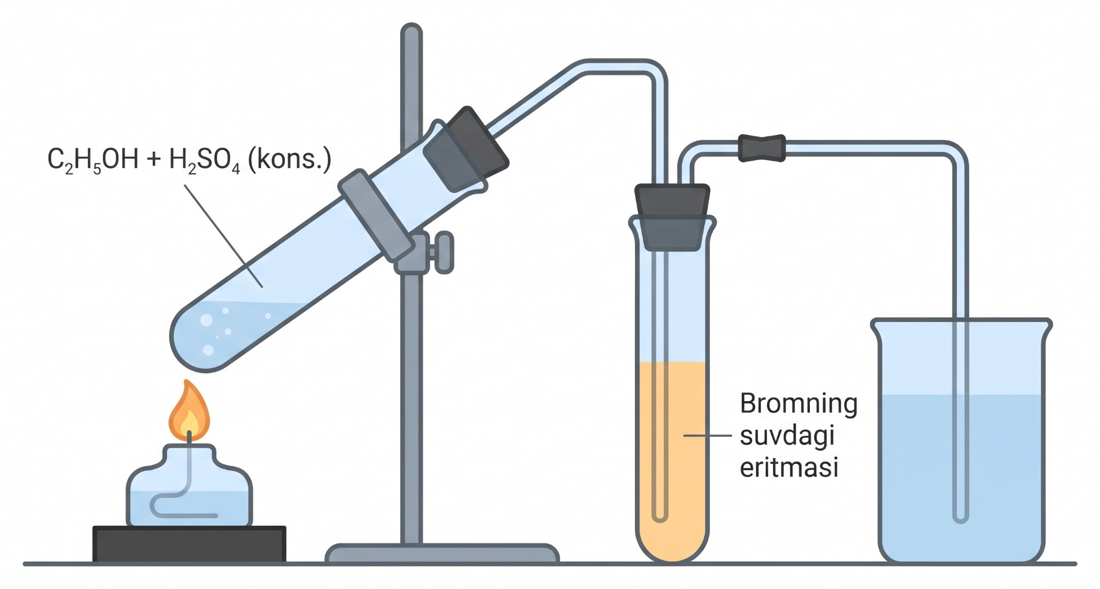
\includegraphics[width=0.86\linewidth]{rasmlar/darslik/d_etilen.png}\end{center}

\noindent A)~\textsl{11,2} \hfill B)~\textsl{20,16} \hfill C)~\textsl{10,08} \hfill D)~\textsl{5,04}\par
\qsep
\noindent\qn{32.} Benzol va toluol eritmalarini (moddalarini) bir-biridan qaysi reagent yordamida farqlash mumkin?
\noindent A)~\textsl{brom suvi}\par
\noindent B)~\textsl{FeCl\textsubscript{3} eritmasi}\par
\noindent C)~\textsl{kislotali KMnO\textsubscript{4} eritmasi (qizdirilganda)}\par
\noindent D)~\textsl{natriy gidroksid   ---}\par
\qsep
\end{multicols}
\medskip
\noindent\setlength{\fboxsep}{0pt}\fbox{\begin{tabular}{p{0.74\linewidth}|p{0.2\linewidth}}
\parbox[t]{0.72\linewidth}{\vspace{3pt}\textbf{Topshiriqlar (33--35) va javob variant (A--F)larini o`zaro to`g`ri moslashtiring.} 0,4 mol/l li AgNO\textsubscript{3} eritmasining 500 ml i inert elektrodlar yordamida 5 A tok kuchi bilan 965 s elektroliz qilindi (eritma hajmi o`zgarmadi deb hisoblang), so`ngra eritmaga mo`l NaCl eritmasi qo`shildi.
\vspace{3pt}} & \parbox[t]{0.19\linewidth}{\vspace{3pt}A~\textsl{0,5}\\[3pt]
B~\textsl{5,4}\\[3pt]
C~\textsl{1}\\[3pt]
D~\textsl{4,32}\\[3pt]
E~\textsl{21,53}\\[3pt]
F~\textsl{10,8}}\\ \hline
\parbox[t]{0.72\linewidth}{\vspace{2pt}\textbf{33. Katodda ajralgan kumush massasini (g) aniqlang.}\vspace{2pt}} & \\ \hline
\parbox[t]{0.72\linewidth}{\vspace{2pt}\textbf{34. Elektrolizdan keyin (NaCl qo`shilishidan oldin) eritmaning pH ini toping.}\vspace{2pt}} & \\ \hline
\parbox[t]{0.72\linewidth}{\vspace{2pt}\textbf{35. NaCl qo`shilganda hosil bo`lgan cho`kma massasini (g) hisoblang.}\vspace{2pt}} & 
\end{tabular}}
\par\bigskip
\noindent\qn{36.} 15\% li va 10\% li tuz eritmalari massalar nisbati 1 : 1 bo`lgan holda aralashtirildi. Tajriba laboratoriyada, shisha idishda o`tkazildi. Hosil bo`lgan eritmaning massa \textbf{ulushini (\%) hisoblang.}
\javob\qsep
\noindent\qn{37.} CuCl\textsubscript{2} eritmasi inert elektrodlar yordamida 4 A tok kuchi bilan 965 s elektroliz qilindi. Katodda ajralgan Cu massasi (g) \textbf{ni toping.}
\javob\qsep
\noindent\qn{38.} Oksidlanish darajasi +2 bo`lgan noma'lum \textit{X} metallning xloridi 11,1 g massada mo`l AgNO\textsubscript{3} eritmasi bilan ta'sirlashganda 28,7 g cho`kma hosil bo`ldi. Reagent (AgNO\textsubscript{3}) eritmasining massa ulushi 50\% va zichligi 1,4 g/ml; u mo`l miqdorda olingan. \textit{X} metallning nisbiy atom \textbf{massasini toping.}
\javob\qsep
\noindent\qn{39.} 14,8 g metilatsetat mo`l NaOH bilan qizdirilganda uning 1/2 qismi gidrolizlandi. Hosil bo`lgan spirt to`liq yondirildi. Reagent (NaOH) eritmasining massa ulushi 36\% va zichligi 1,4 g/ml; u mo`l miqdorda olingan. Yondirishda ajralgan CO\textsubscript{2} \textbf{hajmini (l, n.sh.) toping.}
\javob\qsep
\noindent\qn{40.} 61,5 g nitrobenzol anilinga qaytarildi (unum 90\%), hosil bo`lgan anilin mo`l bromli suv bilan reaksiyaga kirishdi (unum 80\%). Hosil bo`lgan 2,4,6-tribromanilin (M = 330 g/mol) \textbf{massasini (g) toping.}
\javob\qsep
\par\bigskip\begin{center}\textbf{\fontsize{13}{15}\selectfont YOZMA ISH}\end{center}
\noindent\qn{41.} \textbf{Topshiriqni bajarish jarayonida barcha reaksiya tenglamalarini yozing. Miqdoriy va arifmetik hisoblashlarni (unga asos bo`lgan usul yoki formulani ko`rsatgan holda) uzviy ketma-ketlikda bajaring.}\par\smallskip
Mis va magniy kukunlaridan iborat aralashmada mis va magniyning mol nisbati 2 : 1. Aralashma havoda to`liq oksidlanganda uning massasi 4,8 g ga ortdi. Hosil bo`lgan oksidlar 10\% li sulfat kislotaning stexiometrik miqdorida eritildi. Olingan eritma inert elektrodlar yordamida 10 A tok kuchi bilan 7720 s elektroliz qilindi (jarayonda Cu\textsuperscript{2+} to`liq tugadi va suv ham elektrolizga uchradi).\par
\noindent 1)\ Barcha jarayonlarning reaksiya tenglamalarini yozing va tenglashtiring. Dastlabki aralashmadagi mis va magniyning massalarini (g) aniqlang.\par
\noindent 2)\ Oksidlanishga sarflangan kislorodning hajmini (l, n.sh.) va kislota eritmasining massasini (g) hisoblang.\par
\noindent 3)\ Oksidlar erigandan keyingi eritmada CuSO\textsubscript{4} va MgSO\textsubscript{4} ning massa ulushlarini (\%) toping.\par
\noindent 4)\ Elektrolizda katodda ajralgan mis massasini (g) va vodorod hajmini (l, n.sh.) hisoblang. Anodda ajralgan gaz hajmini (l, n.sh.) toping.\par
\noindent 5)\ Elektroliz tugagach eritmadagi MgSO\textsubscript{4} va H\textsubscript{2}SO\textsubscript{4} ning massa ulushlarini (\%) aniqlang.\par
\diqqat{Mazkur topshiriq kengaytirilgan javobni talab etib, uning yechilish usuli va shu usul asosidagi barcha hisoblash amallari javoblar varaqasida aks etishi lozim.}\qsep
\noindent\qn{42.} Quyidagi o`zgarishlar zanjirida \textit{X}, \textit{Y}, \textit{Z} noma'lum organik moddalar:\par
\[\setlength{\fboxsep}{0pt}\text{CH\textsubscript{4}}\xrightarrow{\text{Cl\textsubscript{2}, yorug`lik}}\text{\textit{X}}\xrightarrow{\text{Na}}\text{\textit{Y}}\xrightarrow{\text{Cl\textsubscript{2}, yorug`lik}}\text{\textit{Z}}\xrightarrow{\text{KOH (suvli)}}\text{C\textsubscript{2}H\textsubscript{5}OH}\]
\noindent 1)\ CH\textsubscript{4} $\to$ \textit{X} : reaksiya tenglamasini yozing; hosil bo`lgan moddani nomlang.\par
\noindent 2)\ \textit{X} $\to$ \textit{Y} : reaksiya tenglamasini yozing; hosil bo`lgan moddani nomlang.\par
\noindent 3)\ \textit{Y} $\to$ \textit{Z} : reaksiya tenglamasini yozing; hosil bo`lgan moddani nomlang.\par
\noindent 4)\ \textit{Z} $\to$ C\textsubscript{2}H\textsubscript{5}OH : reaksiya tenglamasini yozing; hosil bo`lgan moddani nomlang.\par
\diqqat{Mazkur topshiriq kengaytirilgan javobni talab etib, uning yechilish usuli va shu usul asosidagi barcha hisoblash amallari javoblar varaqasida aks etishi lozim.}\qsep
\noindent\qn{43.} \textbf{Topshiriqni bajarish jarayonida barcha reaksiya tenglamalarini yozing. Miqdoriy va arifmetik hisoblashlarni (unga asos bo`lgan usul yoki formulani ko`rsatgan holda) uzviy ketma-ketlikda bajaring.}\par\smallskip
Alyuminiy va noma'lum \textit{X} metalldan (\textit{X} -- oksidlanish darajasi +2 bo`lgan metall) iborat 19,5 g aralashma mo`l NaOH eritmasi bilan ta'sirlashganda 3,36 l (n.sh.) gaz ajraldi. Shunday massali ikkinchi namuna mo`l xlorid kislotada eritilganda 10,08 l (n.sh.) gaz ajraldi. Xlorid kislotali eritmaga mo`l NaOH eritmasi qo`shilib, cho`kma ajratildi, havoda to`liq oksidlanguncha tutildi va kuydirildi; filtratdan mo`l CO\textsubscript{2} o`tkazildi. Reagent (NaOH) eritmasining massa ulushi 36\% va zichligi 1,05 g/ml; u mo`l miqdorda olingan. Hosil bo`lgan Al(OH)\textsubscript{3} nitrat kislotada eritildi, eritma bug`latilib, qoldiq doimiy massagacha qizdirildi, ajralgan gazlar suvga yuttirildi.\par
\noindent 1)\ Barcha reaksiyalarning tenglamalarini yozing va tenglashtiring.\par
\noindent 2)\ Aralashmadagi Al va \textit{X} ning miqdorlarini (mol) aniqlang va \textit{X} metallni toping.\par
\noindent 3)\ Aralashmadagi metallarning massa ulushlarini (\%) hisoblang. Al(OH)\textsubscript{3} ni eritish uchun sarflangan HNO\textsubscript{3} miqdorini (mol) toping.\par
\noindent 4)\ Kuydirishdan hosil bo`lgan qattiq moddaning formulasini aniqlang va massasini (g) hisoblang. Al(NO\textsubscript{3})\textsubscript{3} qizdirilganda ajralgan gazlar hajmini (l, n.sh.) hisoblang.\par
\noindent 5)\ Filtratdan CO\textsubscript{2} o`tkazilganda hosil bo`lgan cho`kma massasini (g) toping. Gazlar suvga yuttirilganda hosil bo`lgan HNO\textsubscript{3} massasini (g) aniqlang.\par
\diqqat{Mazkur topshiriq kengaytirilgan javobni talab etib, uning yechilish usuli va shu usul asosidagi barcha hisoblash amallari javoblar varaqasida aks etishi lozim.}\qsep
\newpage
\noindent\textbf{\fontsize{13}{15}\selectfont 6-variant}\hfill \textbf{Javoblar kaliti}\par\smallskip\hrule\smallskip
\textit{Faqat o`qituvchi uchun.}\par\medskip
\noindent\textbf{1--32-savollar}\par\smallskip
\noindent\begin{tabular}{|c|c|c|c|c|c|c|c|c|c|c|c|c|c|c|c|}\hline
\textbf{1} & \textbf{2} & \textbf{3} & \textbf{4} & \textbf{5} & \textbf{6} & \textbf{7} & \textbf{8} & \textbf{9} & \textbf{10} & \textbf{11} & \textbf{12} & \textbf{13} & \textbf{14} & \textbf{15} & \textbf{16}\\\hline
\textsl{A} & \textsl{B} & \textsl{C} & \textsl{A} & \textsl{C} & \textsl{D} & \textsl{D} & \textsl{D} & \textsl{C} & \textsl{A} & \textsl{A} & \textsl{B} & \textsl{B} & \textsl{C} & \textsl{D} & \textsl{D}\\\hline
\textbf{17} & \textbf{18} & \textbf{19} & \textbf{20} & \textbf{21} & \textbf{22} & \textbf{23} & \textbf{24} & \textbf{25} & \textbf{26} & \textbf{27} & \textbf{28} & \textbf{29} & \textbf{30} & \textbf{31} & \textbf{32}\\\hline
\textsl{B} & \textsl{C} & \textsl{A} & \textsl{D} & \textsl{B} & \textsl{B} & \textsl{A} & \textsl{A} & \textsl{D} & \textsl{B} & \textsl{D} & \textsl{C} & \textsl{B} & \textsl{A} & \textsl{C} & \textsl{C}\\\hline
\end{tabular}\par\medskip
\noindent\textbf{33--35-savollar}\par\smallskip
\noindent\begin{tabular}{|c|c|c|}\hline \textbf{No} & \textbf{Javob} & \textbf{Qiymat}\\\hline
33 & \textsl{B} & 5,4\\\hline
34 & \textsl{C} & 1\\\hline
35 & \textsl{E} & 21,53\\\hline
\end{tabular}\par\medskip
\noindent\textbf{36--40-savollar}\par\smallskip
\noindent\begin{tabular}{|c|c|}\hline \textbf{No} & \textbf{To`g`ri javob}\\\hline
36 & 12,5\\\hline
37 & 1,28\\\hline
38 & 40\\\hline
39 & 2,24\\\hline
40 & 118,8\\\hline
\end{tabular}\par\medskip
\noindent\textbf{41--43-topshiriqlar: javoblar}\par\smallskip
\noindent\textbf{41-topshiriq.}\par
\noindent 1) 12,8 g; 2,4 g\par
\noindent 2) 3,36 l; 294 g\par
\noindent 3) 10,19\%; 3,82\%\par
\noindent 4) 12,8 g; 0,2 mol = 4,48 l; 4,48 l\par
\noindent 5) 4,08\%; 6,66\%\par
\noindent\textbf{42-topshiriq.}\par
\noindent 1) CH\textsubscript{4} + Cl\textsubscript{2}, yorug`lik $\to$ CH\textsubscript{3}Cl (xlormetan)\par
\noindent 2) CH\textsubscript{3}Cl + Na $\to$ C\textsubscript{2}H\textsubscript{6} (etan)\par
\noindent 3) C\textsubscript{2}H\textsubscript{6} + Cl\textsubscript{2}, yorug`lik $\to$ C\textsubscript{2}H\textsubscript{5}Cl (xloretan)\par
\noindent 4) C\textsubscript{2}H\textsubscript{5}Cl + KOH (suvli) $\to$ C\textsubscript{2}H\textsubscript{5}OH (etanol)\par
\noindent\textbf{43-topshiriq.}\par
\noindent 1) 2Al + 2NaOH + 6H\textsubscript{2}O $\to$ 2Na[Al(OH)\textsubscript{4}] + 3H\textsubscript{2}$\uparrow$; 2Al + 6HCl $\to$ 2AlCl\textsubscript{3} + 3H\textsubscript{2}$\uparrow$; \textit{X} + 2HCl $\to$ XCl\textsubscript{2} + H\textsubscript{2}$\uparrow$; AlCl\textsubscript{3} + 4NaOH $\to$ Na[Al(OH)\textsubscript{4}]\par
\noindent 2) 0,1 mol; 0,3 mol; Fe\par
\noindent 3) 13,8\%; 86,2\%; 0,3 mol\par
\noindent 4) Fe\textsubscript{2}O\textsubscript{3}; 24 g; 8,4 l\par
\noindent 5) 7,8 g; 18,9 g\par
\par\bigskip\noindent\textbf{Mavzular taqsimoti}\par\smallskip
{\small\noindent\begin{longtable}{|c|p{7.2cm}|p{5.4cm}|c|}\hline \textbf{No} & \textbf{Mavzu} & \textbf{Tekshiriladigan ko`nikma} & \textbf{Ball}\\\hline
1 & 8-sinf; Tirkashev II bob (kimyoviy bog`lanish) & Bilim va tushunish & 1\\\hline
2 & 8-sinf (kristall panjaralar) & Rasm bo`yicha tahlil & 1\\\hline
3 & 11-sinf 8-bob; Tirkashev \textit{V} bob (elektroliz) & Bilim va tushunish & 1\\\hline
4 & Tirkashev I bob; 8-sinf (elektron konfiguratsiya) & Bilim va tushunish & 1\\\hline
5 & Tirkashev I bob; 8-sinf (izoelektron) & Bilim va tushunish & 1\\\hline
6 & 11-sinf (yadro) & Grafik tahlili & 1\\\hline
7 & Tirkashev \textit{V} bob; 11-sinf 7-bob (OQR tenglash) & Hisoblash va masala yechish & 1\\\hline
8 & 9-sinf (metallarning kuchlanish qatori; plastinka massasi o`zgarishi) & Hisoblash va masala yechish & 1\\\hline
9 & 8-sinf (ekvivalentlar qonuni) & Hisoblash va masala yechish & 1\\\hline
10 & 8-sinf; Tirkashev VI bob (Vant-Goff) & Hisoblash va masala yechish & 1\\\hline
11 & Tirkashev VI bob (tezlik, jadval) & Jadval tahlili & 1\\\hline
12 & Tirkashev III bob (eruvchanlik, jadval) & Jadval tahlili & 1\\\hline
13 & 9-11-sinf (gaz hajmi o`zgarishi; parchalanish darajasi) & Hisoblash va masala yechish & 1\\\hline
14 & 9-sinf; Tashev (anorganik birikmalar xossalari) & Bilim va tushunish & 1\\\hline
15 & Tashev (HNO\textsubscript{3} olinishi) & Hisoblash va masala yechish & 1\\\hline
16 & 9-sinf (ion reaksiyalar, anionlarni aniqlash) & Bilim va tushunish & 1\\\hline
17 & 9-sinf (kremniy va uning oksidi) & Hisoblash va masala yechish & 1\\\hline
18 & 9-sinf; 10-sinf (kalsiy; karbidlar) & Hisoblash va masala yechish & 1\\\hline
19 & 9-sinf (azot oksidlari; gaz hajmlari) & Hisoblash va masala yechish & 1\\\hline
20 & 10-sinf (mavzuga oid paragraflar); Abdusamatov & Bilim va tushunish & 1\\\hline
21 & 10-sinf (mavzuga oid paragraflar); Abdusamatov & Bilim va tushunish & 1\\\hline
22 & 10-sinf (organik birikmalar sinflari) & Bilim va tushunish & 1\\\hline
23 & 10-sinf (arenlar, anilin olinishi) & Hisoblash va masala yechish & 1\\\hline
24 & 10-sinf (aldegidlarning kumush ko`zgu reaksiyasi) & Hisoblash va masala yechish & 1\\\hline
25 & 10-sinf (uglevodlar; glukozaning bijg`ishi) & Hisoblash va masala yechish & 1\\\hline
26 & 10-sinf (uglevodorodlarning yonishi) & Hisoblash va masala yechish & 1\\\hline
27 & 10-sinf (aminokislotalar, peptidlar) & Hisoblash va masala yechish & 1\\\hline
28 & 10-sinf (spirtlar, alkenlar, ko`p atomli spirtlar) & Hisoblash va masala yechish & 1\\\hline
29 & 10-sinf (nitrobirikmalar, aminlar) & Hisoblash va masala yechish & 1\\\hline
30 & 7-sinf (laboratoriya jihozlari) & Bilim va tushunish & 1\\\hline
31 & 10-sinf (etilen olinishi, 6-rasm) & Rasm bo`yicha tahlil & 1\\\hline
32 & 9-sinf; 10-sinf (sifat reaksiyalari; moddalarni farqlash) & Bilim va tushunish & 1\\\hline
33--35 & Aralash masala (moslashtirish) & Ko`p bosqichli hisob & 3\\\hline
36--40 & Qisqa javobli masalalar & Hisoblash & 5\\\hline
41--43 & Yozma ish & Usul va hisob (M, A) & 75\\\hline
\end{longtable}}
\end{document}
